\documentclass{report}
\usepackage{tikz}
%\usetikzlibrary{positioning, fit, backgrounds, calc}
\usetikzlibrary{positioning, backgrounds, fit}

\begin{document}

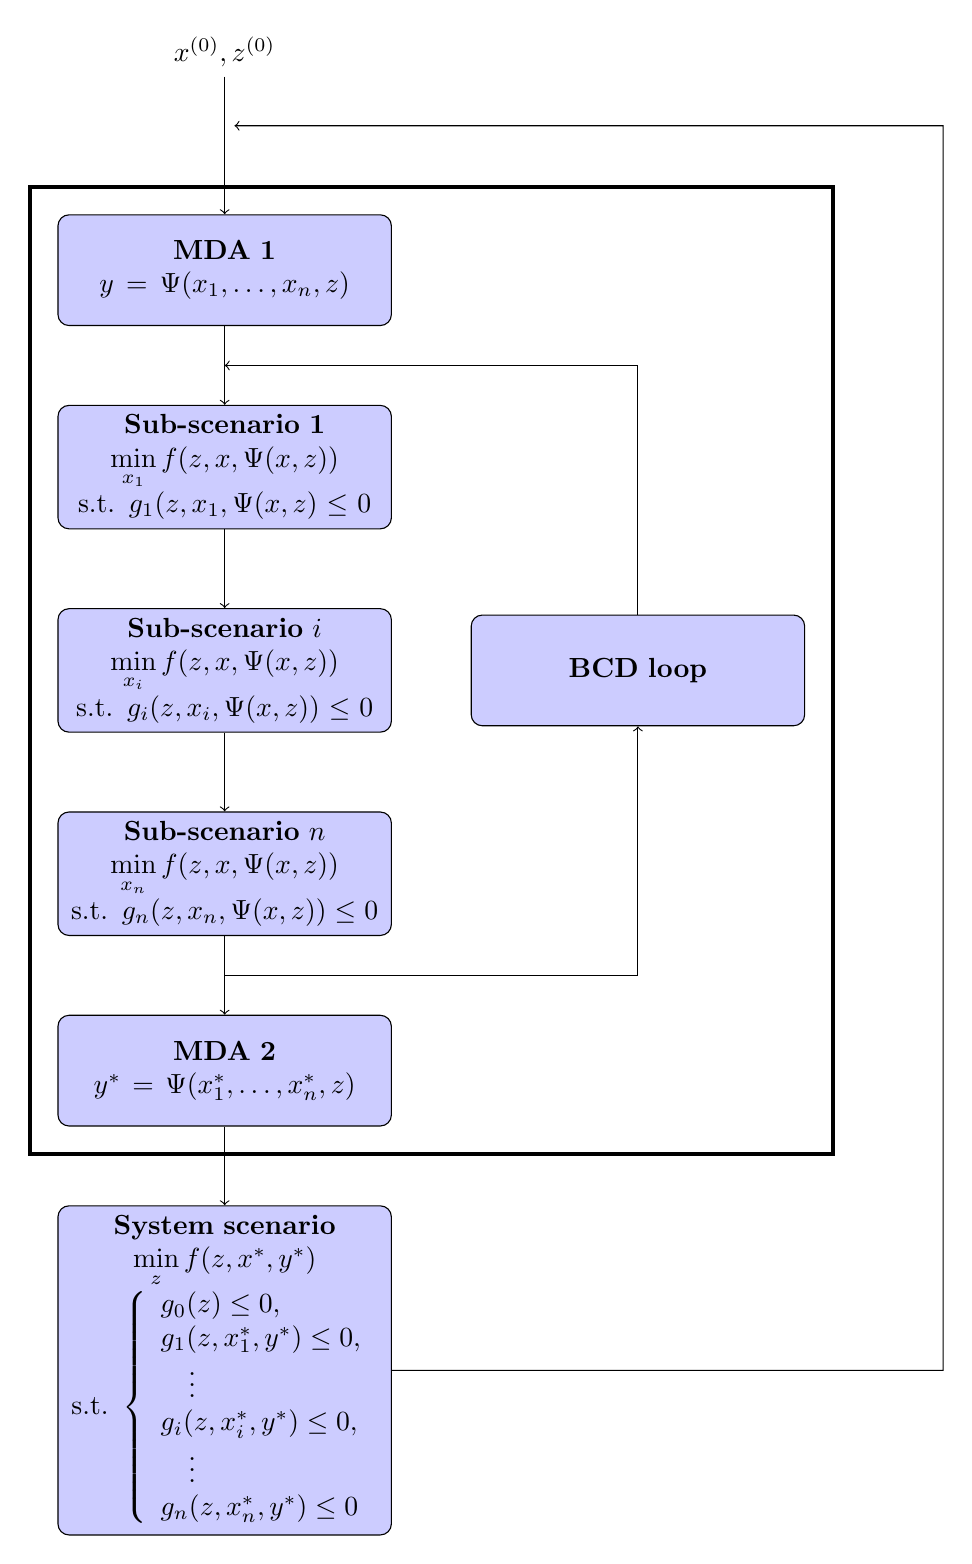
\begin{tikzpicture}[
    node distance=1cm,
    block/.style={rectangle, draw, fill=blue!20, text width=4cm, text centered, rounded corners, minimum height=4em},
]

% Nodes
\node [block] (min1) {\textbf{Sub-scenario 1} \\ $\min\limits_{x_1} f(z, x, \Psi(x, z))$ \\ s.t. $g_1(z, x_1, \Psi(x, z) \leq 0$};
\node [block, below=of min1] (mini) {\textbf{Sub-scenario $i$} \\ $\min\limits_{x_i} f(z, x, \Psi(x, z))$ \\ s.t. $g_i(z, x_i, \Psi(x, z)) \leq 0$};
\node [block, below=of mini] (minn) {\textbf{Sub-scenario $n$} \\ $\min\limits_{x_n} f(z, x, \Psi(x, z))$ \\ s.t. $g_n(z, x_n, \Psi(x, z)) \leq 0$};
\node [block, below=of minn] (mda2) {\textbf{MDA 2} \\ $y^* = \Psi(x_1^*, \ldots, x_n^*, z)$};
\node [block, below=of mda2] (min_sys) {\textbf{System scenario} \\ $\min\limits_{z} f(z, x^*, y^*)$ \\ s.t. $\left\{\begin{array}{l}
                                g_0(z) \leq 0, \\
                                g_1(z, x_1^*, y^*) \leq 0, \\
                                \quad\vdots \\
                                g_i(z, x_i^*, y^*) \leq 0, \\
                                \quad\vdots \\
                                g_n(z, x_n^*, y^*) \leq 0
                                \end{array}\right.$};
\node [block, above=of min1] (mda1) {\textbf{MDA 1} \\ $y = \Psi(x_1, \ldots, x_n, z)$};
\node [block, right=of mini] (bcd) {\textbf{BCD loop}};


\node [above=1cm of mda1] (tmp1) {};
\node [above=0.5cm of tmp1] (x0) {$x^{(0)}, z^{(0)}$};
\node [right=5cm of min_sys] (tmp2) {};
\node [right=5cm of tmp1] (tmp3) {};

% Lines
\path [->] (mda1) edge (min1);
\path [->] (min1) edge (mini);
\path [->] (mini) edge (minn);
\path [->] (minn) edge (mda2);
\path [->] (mda2) edge (min_sys);
\path [->] (x0) edge (mda1);
\draw [->] (min_sys.east) -- ([xshift=7cm]min_sys.east) -- ([xshift=9cm]tmp1.east) --(tmp1.east) ;
\draw [->] ([yshift=-0.5cm]minn.south) -| (bcd.south) ;
\draw [->] (bcd.north) |- ([yshift=0.5cm]min1.north) ;

% Background
\begin{scope}%[on background layer]
    \node [draw, line width=1.5pt, fit=(mda1) (min1) (mini) (minn) (mda2) (bcd), inner sep=1em] (background) {};
\end{scope}


\end{tikzpicture}

\end{document}
